\documentclass[crop, tikz]{standalone}
\usepackage{tikz}


% Colour
\usepackage{xcolor}
\colorlet{LightCyan}{cyan!30}
% Nodes
\tikzstyle{bLSTMblock}=[draw,fill=LightCyan,minimum size=34pt,inner sep=1pt]
\tikzstyle{LSTMblock}=[draw,fill=LightCyan,minimum size=20pt,inner sep=1pt]
\tikzstyle{circle_node}=[draw,circle,minimum size=34pt,inner sep=1pt]
\tikzstyle{invisNode}=[circle, line width=0mm, inner sep=0pt]
\tikzstyle{stateTransition}=[-stealth, thick]
% Reverse direction vector arrow
\usepackage{graphicx}
\newcommand{\cev}[1]{\reflectbox{\ensuremath{\vec{\reflectbox{\ensuremath{#1}}}}}}

\begin{document}
    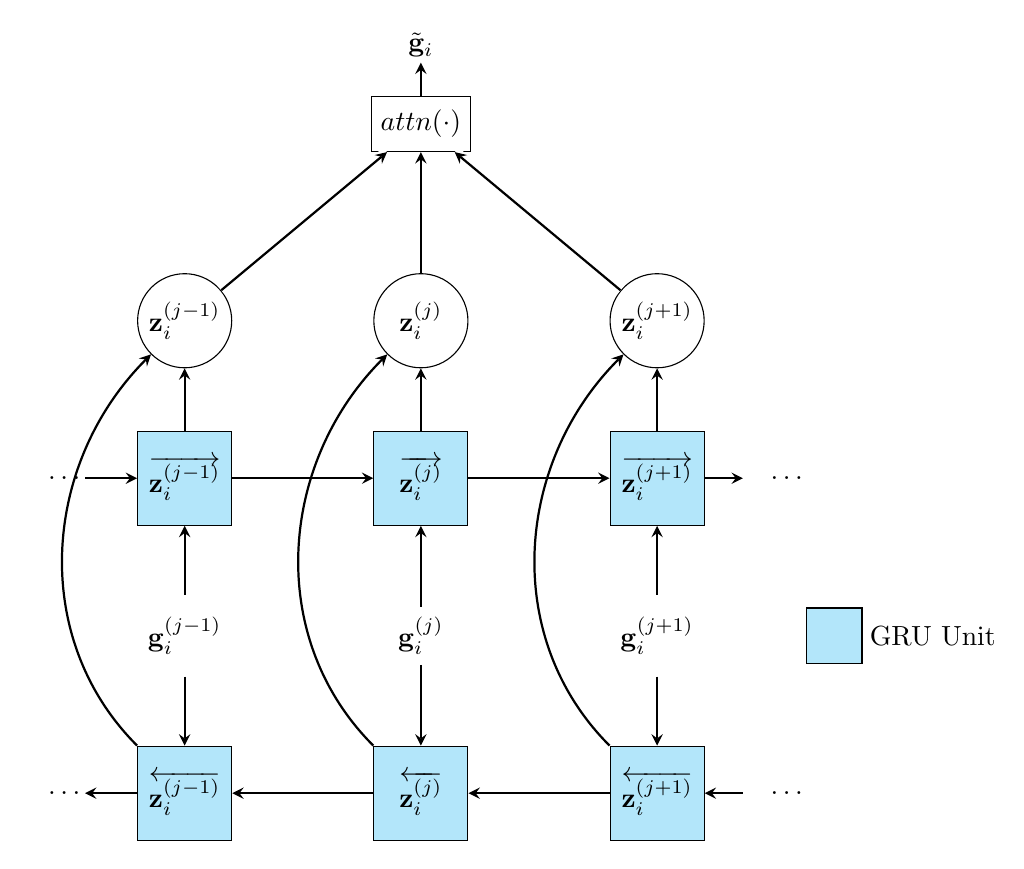
\begin{tikzpicture}
        % Forward Direction
        \node[bLSTMblock] (h0) at (-3, 0) {$\overrightarrow{\mathbf{z}_i^{(j-1)}}$};
        \node[bLSTMblock] (h1) at (0, 0) {$\overrightarrow{\mathbf{z}_i^{(j)}}$};
        \node[bLSTMblock] (h2) at (3, 0) {$\overrightarrow{\mathbf{z}_i^{(j+1)}}$};
        \node[invisNode] (i0) at (-4.5, 0) {\dots \quad};
        \node[invisNode] (i1) at (4.5, 0) {\quad \dots};

        \node[circle_node] (y0) at (-3, 2) {$\mathbf{z}_i^{(j-1)}$};
        \node[circle_node] (y1) at (0, 2) {$\mathbf{z}_i^{(j)}$};
        \node[circle_node] (y2) at (3, 2) {$\mathbf{z}_i^{(j+1)}$};
        
        \node[invisNode] (x0) at (-3, -2) {$\mathbf{g}_i^{(j-1)}$};
        \node[invisNode] (x1) at (0, -2) {$\mathbf{g}_i^{(j)}$};
        \node[invisNode] (x2) at (3, -2) {$\mathbf{g}_i^{(j+1)}$};

    	\draw[stateTransition] (i0) to[out=0,in=180] node [midway, sloped, above] {} (h0);
    	\draw[stateTransition] (h0) to[out=0,in=180] node [midway, sloped, above] {} (h1);
    	\draw[stateTransition] (h1) to[out=0,in=180] node [midway, sloped, above] {} (h2);
    	\draw[stateTransition] (h2) to[out=0,in=180] node [midway, sloped, above] {} (i1);

    	\draw[stateTransition] (x0) to[out=90,in=270] node [midway, sloped, above] {} (h0);
    	\draw[stateTransition] (x1) to[out=90,in=270] node [midway, sloped, above] {} (h1);
    	\draw[stateTransition] (x2) to[out=90,in=270] node [midway, sloped, above] {} (h2);
    	
    	\draw[stateTransition] (h0) to[out=90,in=270] node [midway, sloped, above] {} (y0);
    	\draw[stateTransition] (h1) to[out=90,in=270] node [midway, sloped, above] {} (y1);
    	\draw[stateTransition] (h2) to[out=90,in=270] node [midway, sloped, above] {} (y2);
    	
    	% Backwards direction
        \node[bLSTMblock] (h3) at (-3, -4) {$\overleftarrow{\mathbf{z}_i^{(j-1)}}$};
        \node[bLSTMblock] (h4) at (0, -4) {$\overleftarrow{\mathbf{z}_i^{(j)}}$};
        \node[bLSTMblock] (h5) at (3, -4) {$\overleftarrow{\mathbf{z}_i^{(j+1)}}$};
        \node[invisNode] (i2) at (-4.5, -4) {\dots \quad};
        \node[invisNode] (i3) at (4.5, -4) {\quad \dots};

    	\draw[stateTransition] (h3) to[out=180,in=0] node [midway, sloped, above] {} (i2);
    	\draw[stateTransition] (h4) to[out=180,in=0] node [midway, sloped, above] {} (h3);
    	\draw[stateTransition] (h5) to[out=180,in=0] node [midway, sloped, above] {} (h4);
    	\draw[stateTransition] (i3) to[out=180,in=0] node [midway, sloped, above] {} (h5);
    	
    	\draw[stateTransition] (x0) to[out=270,in=90] node [midway, sloped, above] {} (h3);
    	\draw[stateTransition] (x1) to[out=270,in=90] node [midway, sloped, above] {} (h4);
    	\draw[stateTransition] (x2) to[out=270,in=90] node [midway, sloped, above] {} (h5);
    	
    	\draw[stateTransition] (h3) to[out=135,in=225] node [midway, sloped, above] {} (y0);
    	\draw[stateTransition] (h4) to[out=135,in=225] node [midway, sloped, above] {} (y1);
    	\draw[stateTransition] (h5) to[out=135,in=225] node [midway, sloped, above] {} (y2);
    	
    	\node[LSTMblock] (LSTMLegend) at (5.25, -2) {};
        \node[invisNode] (LSTMtext) at (6.5,-2) {GRU Unit};
        
        % Attention
    	\node[draw, minimum size=20pt] (attn) at (0, 4.5) {$\text{attn}(\cdot)$};
    	\node[invisNode] (g_tilde) at (0, 5.5) {$\tilde{\mathbf{g}}_i$};
    	\draw[stateTransition] (attn) to[out=90,in=270] node [midway, sloped, above] {} (g_tilde);

    	\draw[-, line width=1.5mm, white] (y0) -- (attn);
    	\draw[-stealth, thick] (y0) -- (attn);
    	\draw[-, line width=1.5mm, white] (y1) -- (attn);
    	\draw[-stealth, thick] (y1) -- (attn);
    	\draw[-, line width=1.5mm, white] (y2) -- (attn);
    	\draw[-stealth, thick] (y2) -- (attn);
    \end{tikzpicture}

\end{document}